\section{Onion routing for predictible DTN}\label{sec:proposal}

%\red{Aim of this section: •.}

%\red{Aim of this section: Brief introduction of what are we going to talk about in this section.}

In this section, we define a model of predictable DTNs using dynamic graphs. After that, we propose an algorithm for onion routing path selection process using the contact knowledge of the network.

We need to perform the following steps in order to successfully send an anonymous message:

\begin{itemize}
\item	\textbf{Step 0:} Key exchange process, load of contact knowledge and network setup.
\item \textbf{Step 1:} The source \textit{s} chooses a destination \textit{d}, an instant of time \textit{t} to send the message, the number of routers in the path \textit{n} and the number of paths \textit{k}.
\item \textbf{Step 2: } The source, using the path selection method, obtains a set of paths and choose one path \textit{p} randomly.
\item \textbf{Step 3: } The message is sent from \textit{s} to \textit{d} at time \textit{t} through \textit{p} path using onion routing.
\end{itemize}

\subsection{Contact representation}

% \red{Aim of this section: Explain how we stored the contact information of the network. Explain that we used a dynamic graph, defining what a graph is and what means to mean a dynamic one.} \\

Clearly, we need to use a structure to represent the network activity. One method that seems to work is to use a graph structure as a way of network activity representation \cite{probabilistic-dtn}, \cite{deterministic-dtn}, \cite{contact-graph}. Each node of the network is represented as a graph vertex (or node) and each contact between nodes as a graph edge. 

There is a subset of graphs in the graph theory called \textit{dynamic graphs}. Dynamic graphs allow to represent the evolution of the network during time easily, i.e: nodes and edges may change positions and appear and/or disappear through time. To do so, we can set a pair of attributes that point out when a node appears and disappears.

The network is modelled as a dynamic graph $G=(V,E)$. The set of vertices $V$ is the set of nodes, and the edges $E$ are the contacts between nodes. Dynamic graphs provide a good way to store dynamic information about the network. In our case this information will be related to contacts like the instant of time when the connection opportunity occurs and how long this contact has been.

In figure \ref{fig:dynamic-graph-example} the evolution of a given graph representing different contacts between buses in a public transport network is shown. In this example we can see that at the beginning, no contacts have been produced yet. As the time passes, the contacts (\textit{edges}) appear and disappear between buses (\textit{nodes}). 

\begin{figure}[h!tb]
\centering
  \subfloat[Complete graph]{%
  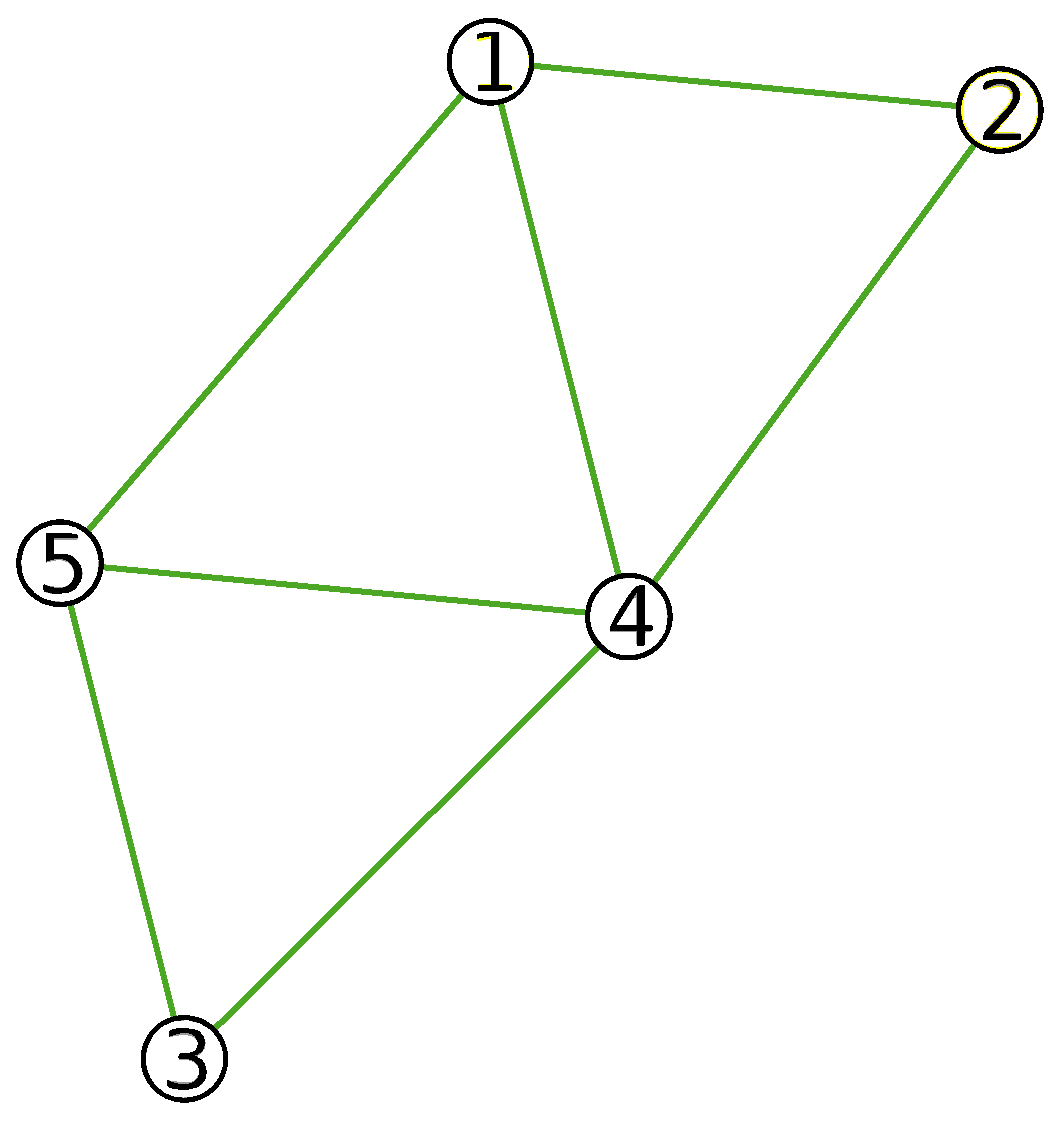
\includegraphics[scale=0.23]{imgs/example-dynamic/full}} \hfill
    \subfloat[$t = 0$]{%
    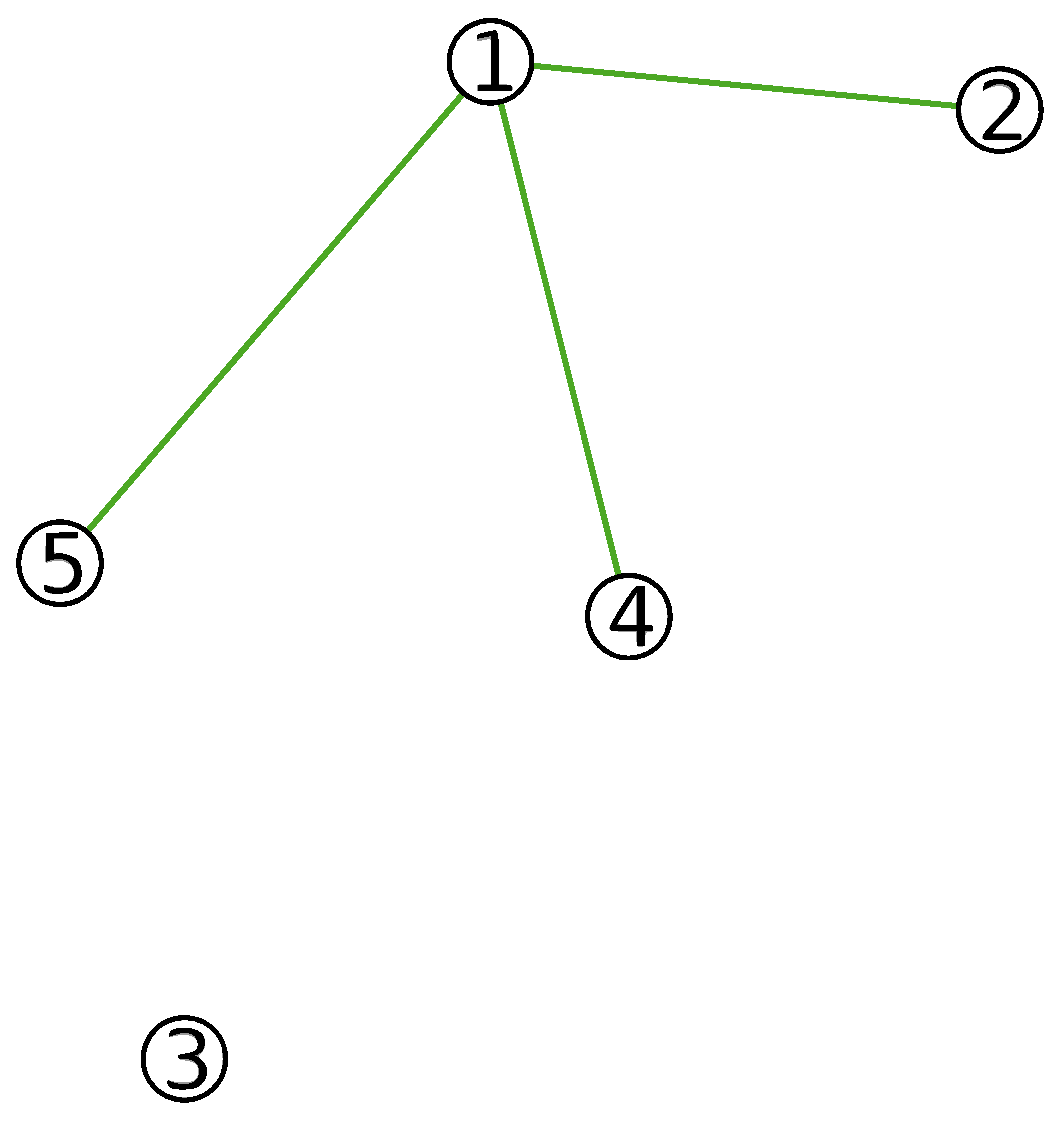
\includegraphics[width=.30\textwidth]{imgs/example-dynamic/t0}}\hfill
  \subfloat[$t = 1$]{%
    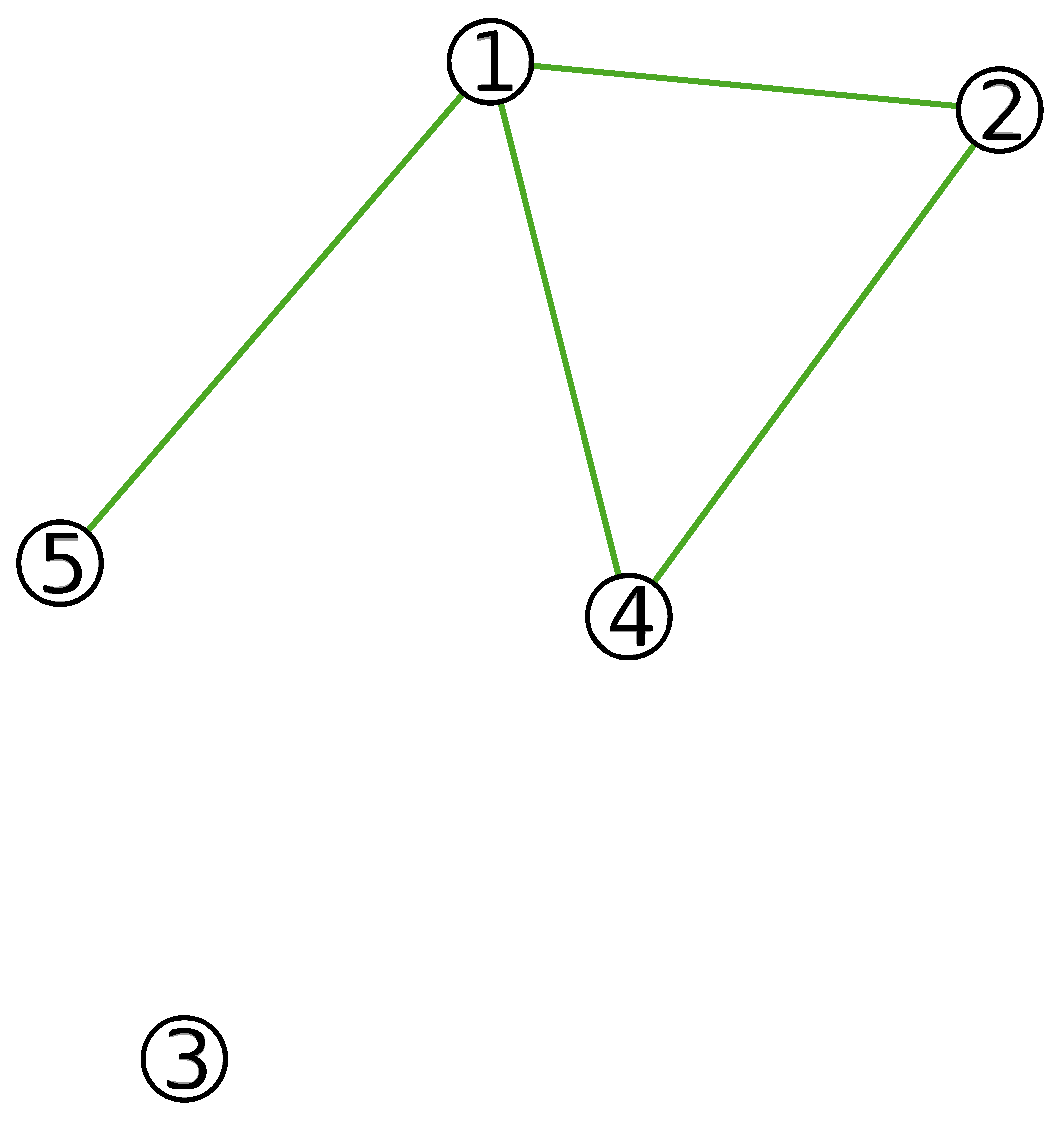
\includegraphics[width=.30\textwidth]{imgs/example-dynamic/t1}}\hfill
    \subfloat[$t = 2$]{%
    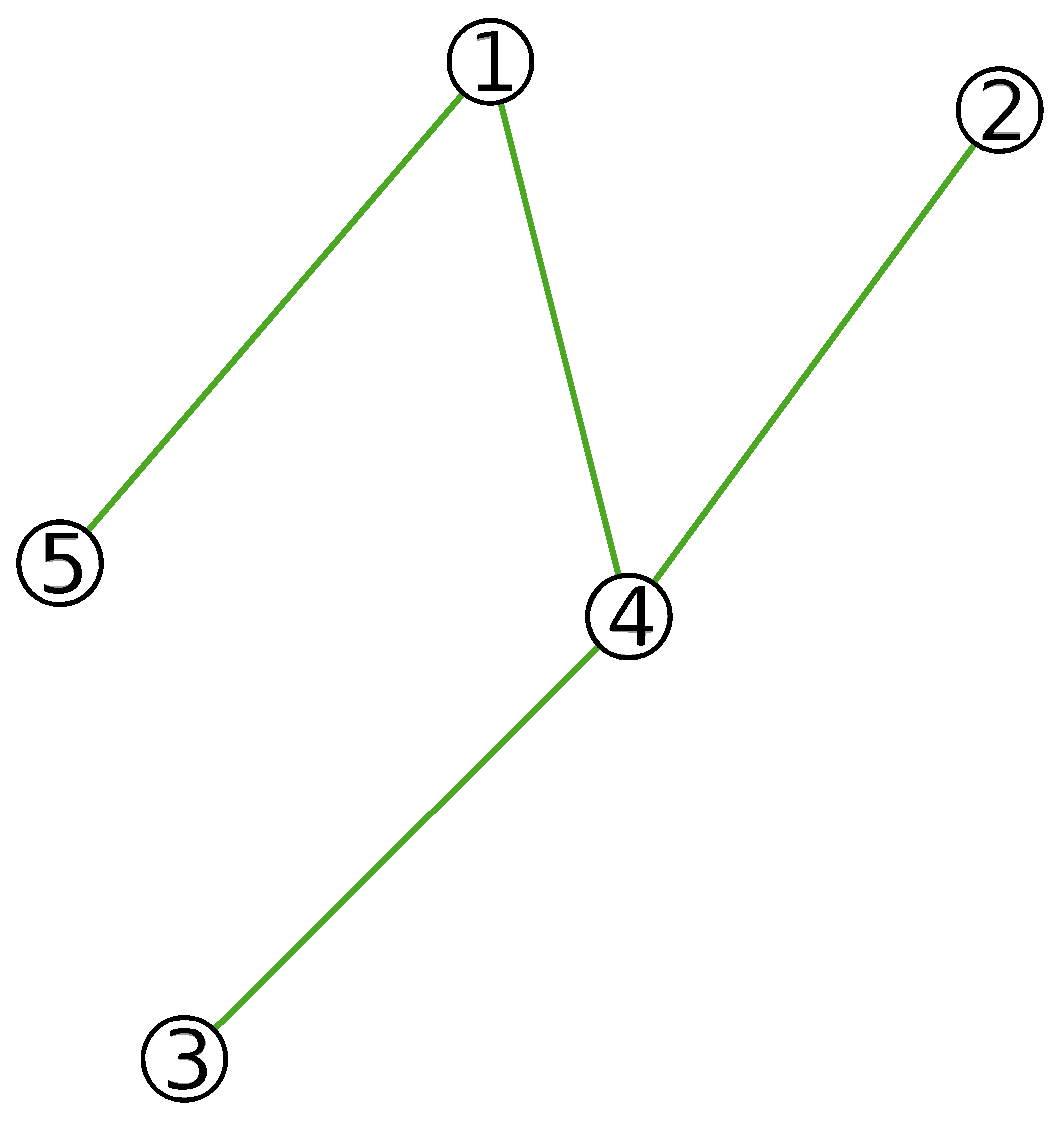
\includegraphics[width=.30\textwidth]{imgs/example-dynamic/t2}}\hfill
  \subfloat[$t = 3$]{%
    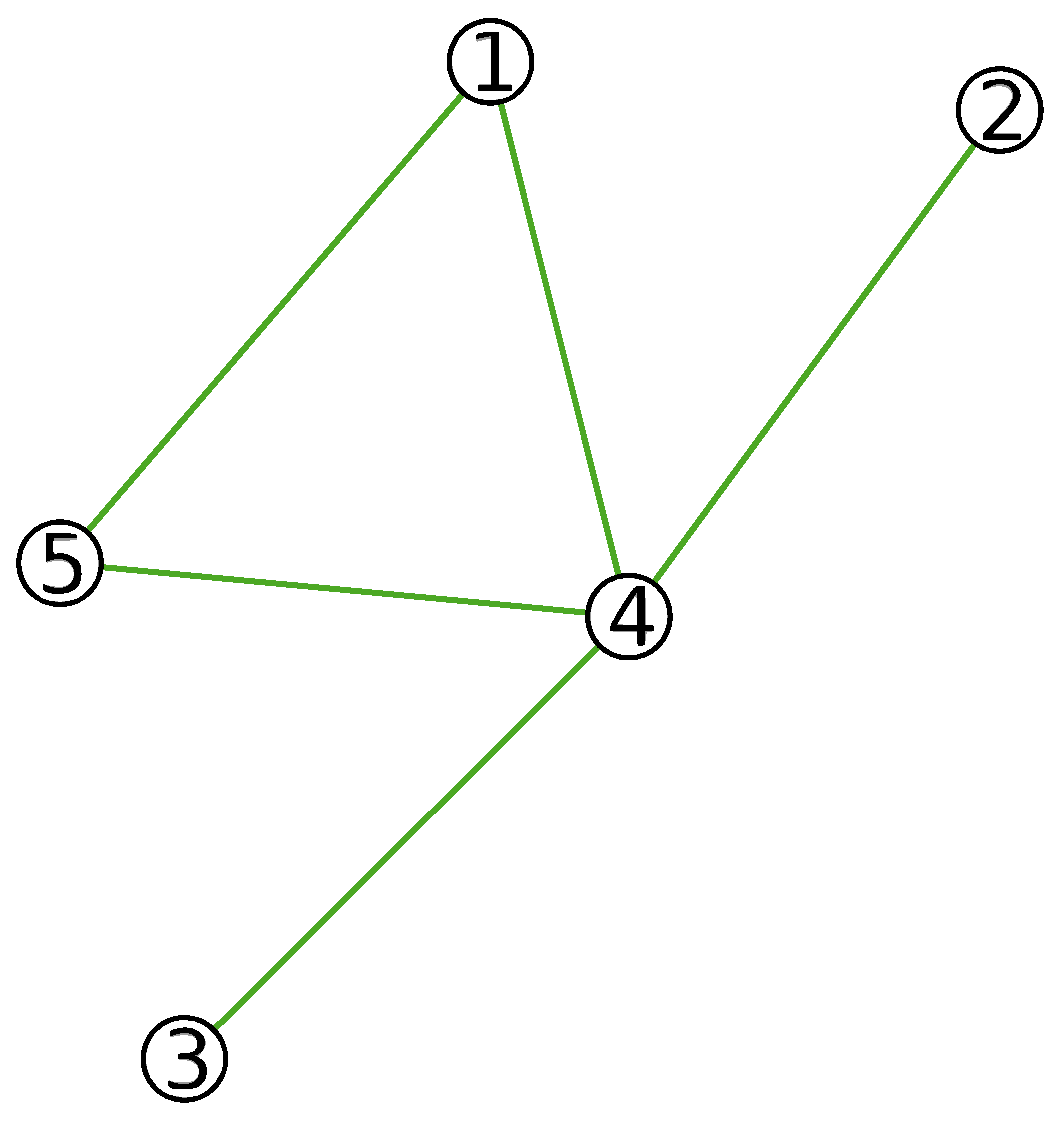
\includegraphics[width=.30\textwidth]{imgs/example-dynamic/t3}} \hfill
  \subfloat[$t = 4$]{%
    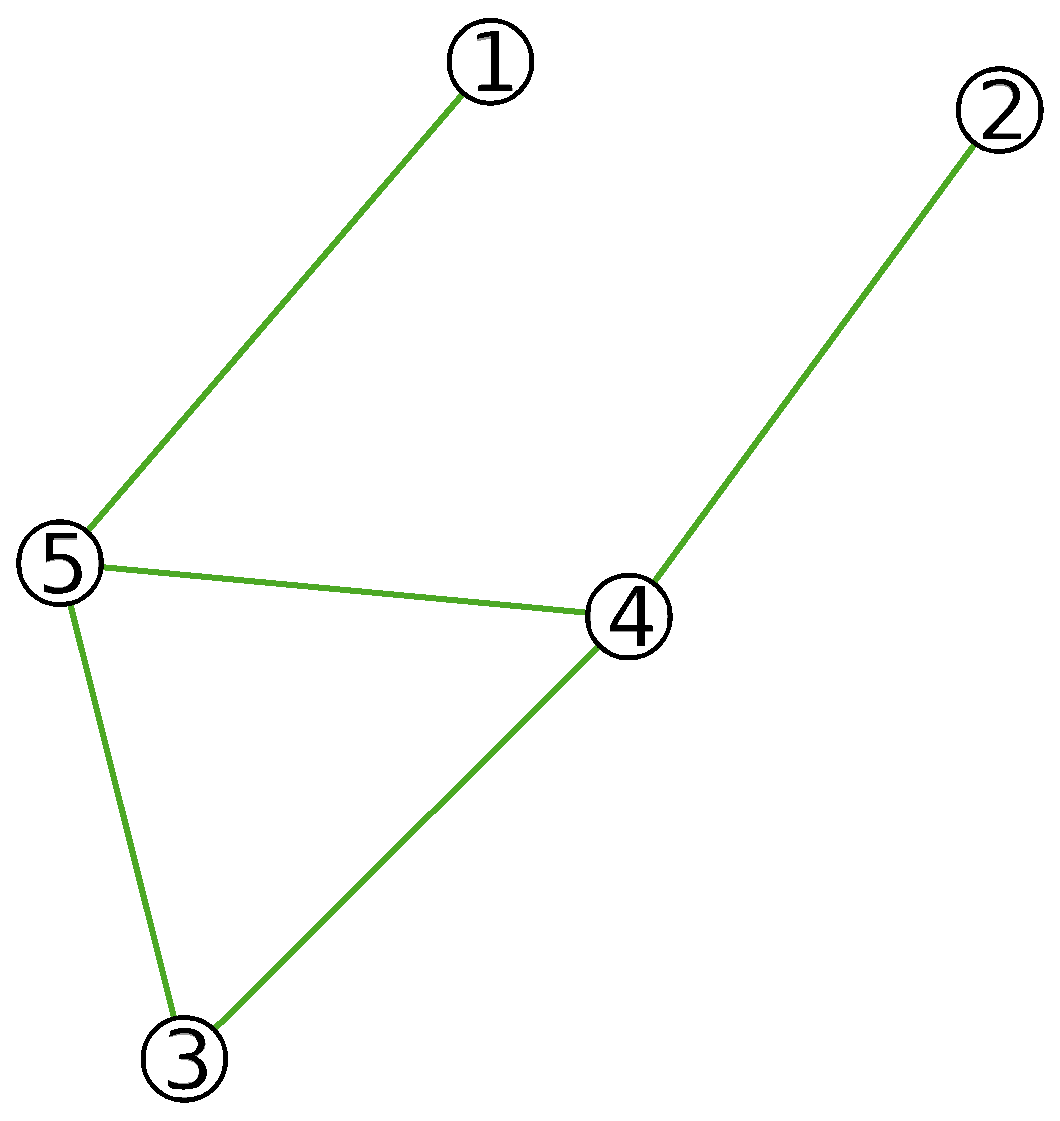
\includegraphics[width=.30\textwidth]{imgs/example-dynamic/t4}}\\
  \subfloat[$t = 5$]{%
    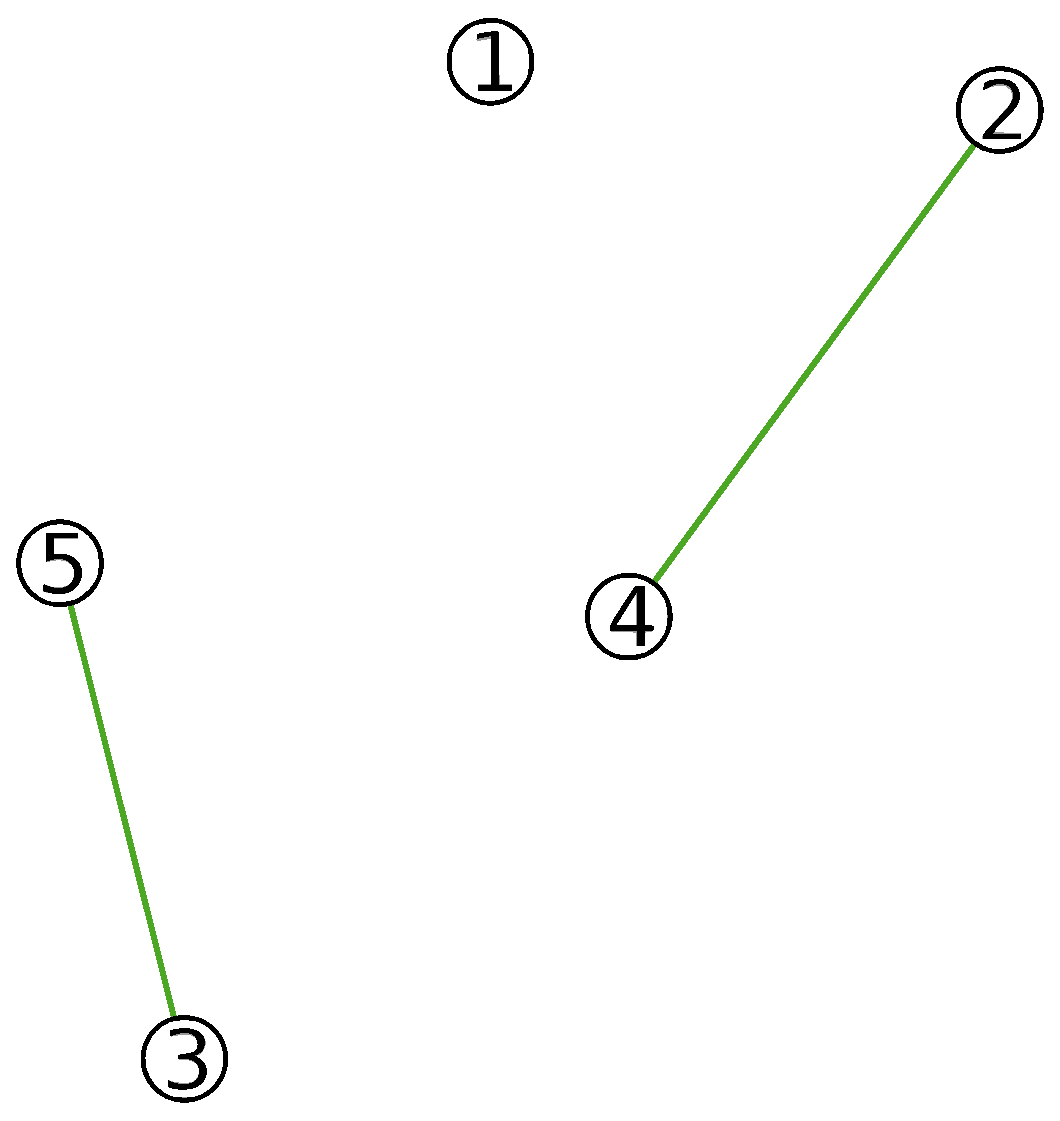
\includegraphics[width=.30\textwidth]{imgs/example-dynamic/t5}}\hfill
    \subfloat[$t = 6$]{%
    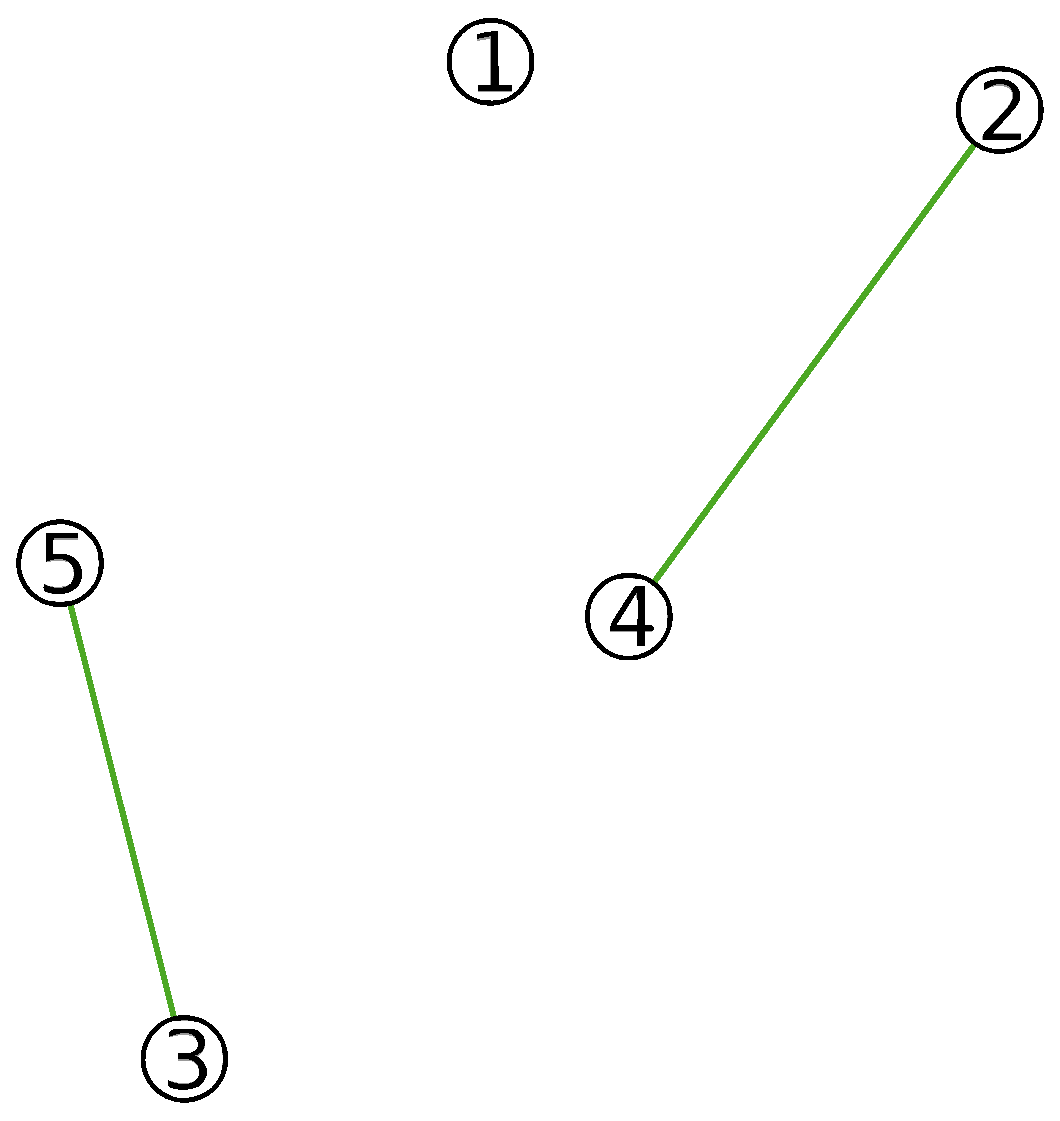
\includegraphics[width=.30\textwidth]{imgs/example-dynamic/t6}}\hfill
  \subfloat[$t = 7$]{%
    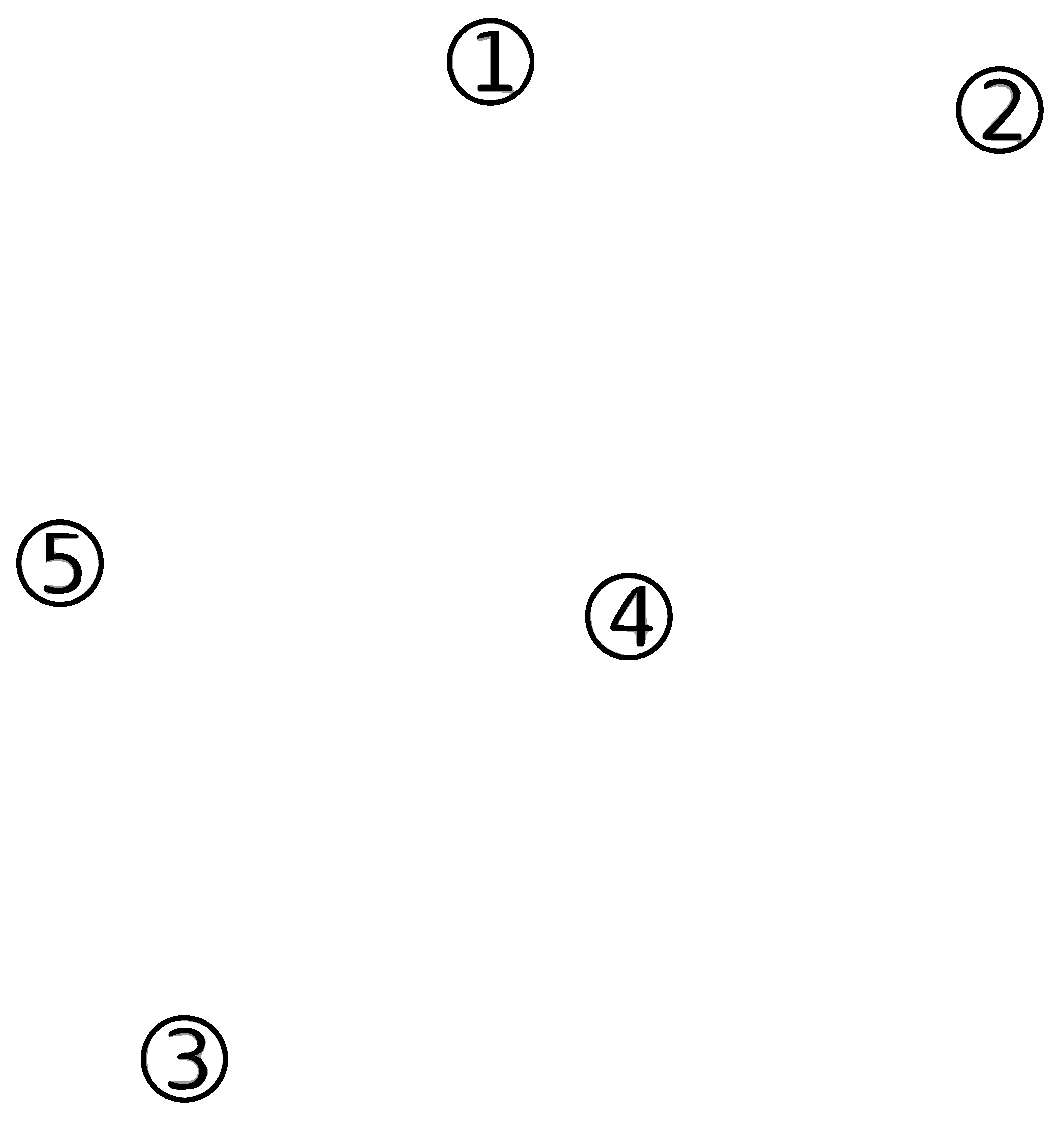
\includegraphics[width=.30\textwidth]{imgs/example-dynamic/t7}} 
  \caption{In $(a)$ the accumulative graph (\textit{t = [0, $+\infty$)}) can be seen. In $(b)-(i)$ different snapshots in given instants of time showing the evolution of the dynamic graph are depicted.}
  \label{fig:dynamic-graph-example}
\end{figure}

\subsection{Path selection}

%\red{Aim of this section: Explain what we did to get some useful paths according to a set of given parameters. Is important to explain the dynamic graph part, the algorithm itself, etc. \textbf{All theoretically!}} \\

Imagine that we have a source node \textit{s} willing to send a message to a destination \textit{d} at time \textit{t} using onion routing. In onion routing you need to choose the number of nodes  \textit{n} where the message will pass through. Node \textit{s} obtains a path to perform the layering process and send the message. The time required to exchange the message between nodes is defined as \textit{tt}. 

To make even harder the path guessing from third parties, as the network knowledge is shared among all nodes, the node \textit{s} obtains a set of paths \textit{k} in order to choose one of them randomly. To sum up, we need a method \textit{f(s, d, t, n, k, tt)} that will retrieve a set of paths to finally choose one following the \textit{t}, \textit{n}, \textit{k} and \textit{tt} requirements. 

The procedures shown in Algorithm~\ref{alg:get-neighbors} and Algorithm~\ref{alg:get-paths} are an example of deterministic choosing for onion routing. Both of them inherit values to filter out unneeded paths. Specifically, in Algorithm~\ref{alg:get-neighbors} from a given node \textit{host} at time \textit{currentTime} we return a set of neighbors  that are available or will be available to forward the message. In Algorithm~\ref{alg:get-paths} we perform a recursive search to get up to \textit{k} paths of length \textit{n} from \textit{source} to \textit{destination}.

In figure~\ref{fig:dynamic-graph-example} there is an example of contact data representation using dynamic graphs. Applying our path selection method with the following parameters: source node \textit{s=1}, destination node \textit{d=5}, starting time \textit{t=0}, number of paths \textit{k=4}, number of nodes of each path \textit{n=5} and transmission time \textit{tt=1}, we get the following paths: \\

\noindent\fbox{%
    \parbox{\textwidth}{%
        \textit{Path: 0} \\
		(1:0) $\rightarrow$ (2:0) $\rightarrow$ (4:1) $\rightarrow$ (1:2) $\rightarrow$ (5:3). Arrival time: 4\\
		\textit{Path: 1}\\
		(1:0) $\rightarrow$ (2:0) $\rightarrow$ (4:1) $\rightarrow$ (3:2) $\rightarrow$ (5:4). Arrival time: 5\\
		\textit{Path: 2}\\
		(1:0) $\rightarrow$ (4:0) $\rightarrow$ (1:1) $\rightarrow$ (4:2) $\rightarrow$ (5:3). Arrival time: 4\\
		\textit{Path: 3}\\
		(1:0) $\rightarrow$ (4:0) $\rightarrow$ (2:1) $\rightarrow$ (4:2) $\rightarrow$ (5:3). Arrival time: 4\\
		
		(node: t): Means forward the message to node at time \textit{t}.
    }%
}\\

So, we get 4 different paths composed by 5 nodes each, i.e: origin and destination plus 3 onion routers, so 3 layers will be performed. From the given set of paths, the source node \textit{s} will need to choose one in order to perform the onion routing itself. To make the guessing of the source node difficult, the path to send the message will be chosen randomly from the given set.

\begin{algorithm}
\caption{Procedure to get valid neighbors of a given node}
\label{alg:get-neighbors}
\begin{algorithmic}[1]
\INHERIT (1) \textit{source}, source node. (2) \textit{destination}, destination node. (3) \textit{t}, when the message will be sent. (4) \textit{k}, maximum number of paths. (5) \textit{n}, number of nodes for each path (including source and destination). (6) \textit{tt}, transmission time required to forward the message.
\INPUT (1) \textit{host}, host node. (2) \textit{currentTime}, current time.
\OUTPUT (1) \textit{validNeighbors}, a set of valid neighbors to whom forward the message.
\Procedure{GetAvailableNeighbors }{host, currentTime}
\ForAll{$\textit{nbr} \in \textit{host.neighbors()}$} 
	\If{$(\textit{nbr}.activationTime + \textit{nbr}.contactDuration - \textit{tt}) \geq \textit{currentTime}$}
		\State $\textit{validNeighbors}.add(\textit{nbr})$
	\EndIf
\EndFor
\State \Return $\textit{validNeighbors}$
\EndProcedure
\end{algorithmic}
\end{algorithm}

\begin{algorithm}
\caption{Procedure to get paths that follows the inherited requirements}
\label{alg:get-paths}
\begin{algorithmic}[1]
\INHERIT (1) \textit{source}, source node. (2) \textit{destination}, destination node. (3) \textit{t}, when the message will be sent. (4) \textit{k}, maximum number of paths. (5) \textit{n}, number of nodes for each path (including source and destination). (6) \textit{tt}, transmission time required to forward the message.
\INPUT (1) \textit{currentPath}, current path. (2) \textit{currentTime}, current time.
\OUTPUT (1) \textit{paths}, a set of paths that follows the inherited requirements.
\Procedure{GetPaths}{currentPath, currentTime}

\If{$\textit{currentPath.size()} \neq \textit{n}$ and $\textit{paths.size()} < \textit{k}$}
	\State $\textit{node} \gets \textit{currentPath.last()}$
	\State $\textit{validNeighbors} \gets \textit{GetAvailableNeighbors(node, currentTime)}$
	\ForAll{$\textit{nbr} \in \textit{validNeighbors}$}
		\State $\textit{oldPath} \gets \textit{currentPath}$
		\State $\textit{nbr.sendingTime} \gets$ max$(\textit{nbr.activationTime}, \textit{currentTime}) + tt$
		\State $\textit{currentPath} \gets \textit{nbr}$
		\If{$\textit{nbr} = \textit{destination}$ and $\textit{currentPath.size()} = \textit{n}$ and $\textit{currentPath} \not\in \textit{paths}$}
			\State $\textit{validNeighbors}.add(\textit{nbr})$
		\Else
			\State \textsc{GetPaths}$(\textit{currentPath}, \textit{nbr.sendingTime})$	\Comment{Recursive part}
		\EndIf
		\State $\textit{currentPath} \gets \textit{oldPath}$
	\EndFor
\EndIf

\State \Return$\textit{paths}$
\EndProcedure
\end{algorithmic}
\end{algorithm}